\documentclass[12pt,a4paper,titlepage]{article}
\usepackage{graphicx}
\usepackage[ngerman]{babel} 
\usepackage[utf8]{inputenc} 
\usepackage{setspace}
\usepackage{tabularx}
\usepackage{acronym}
\usepackage{hyperref}
\usepackage{color}
\usepackage{titlesec}
\usepackage[a4paper,left=2cm,right=2cm,top=3cm,bottom=3cm]{geometry}
\usepackage{wrapfig}
\usepackage{float}
\usepackage{fancyhdr}
\pagestyle{fancy} 
\fancyhf{} 
\renewcommand{\headrulewidth}{0.4pt} 
\renewcommand{\footrulewidth}{0.4pt}
\renewcommand{\sectionmark}[1]{\markright{#1}}
\renewcommand{\subsectionmark}[1]{}
\renewcommand{\subsubsectionmark}[1]{}
\lhead{\nouppercase{\rightmark}}
\rhead{\thepage}
\lfoot{Benjamin Mosberger, Tobias Schoch}



%--------Titelseite----------
\begin{document}
\newgeometry{left=0cm,right=0cm, top=1cm} 
\thispagestyle{empty}
\begin{center}
	
\includegraphics[height=2cm]{logo_ntb.png}
	\hspace*{6cm}
	
\includegraphics[height=1.6cm]{logo_htw.png}\\
	\vspace{5cm}
	\Large{NTB - Interstaatliche Hochschule für Technik Buchs}\\
	\vspace{3cm}
	\Huge{IuK\_III\_U-Konzeption und Aufbau eines Unternehmensnetzwerkes}\\
	\vspace{8cm}
	\Large{}
	\doublespacing
	\begin{tabular}{lll}
		\textbf{Studierende:} & Benjamin Mosberger, &Tobias Schoch \\ 
		\textbf{Dozent:} & Beat Bigger \\
		\textbf{Datum:} & Herbstsemester 2015
	\end{tabular}	
\end{center}
\restoregeometry
\pagebreak

%--------Abstract----------
\setcounter{page}{1}
\onehalfspacing 

\section*{Zusammenfassung}
Die Aufgabe dieser Projektarbeit ist ein Unternehmensnetzwerk im Labor der HTW Chur zu planen, aufzubauen und zu Dokumentieren. Das ganze Netzwerk soll redundant aufgebaut werden, um ausfallsicher zu sein, und ausserdem wird IPv4 und IPv6 verwendet.


\vspace{-1,2em}

\section*{Abstract}
The goal of this project is to achieve a working corporate network. Beside redundancy, the clients should be able to use IPv4 and Ipv6. Clients from a department should only be able to communicate with users from the same department, even in other sites.

\pagebreak

%--------Inhaltsverzeichnis---------- 
\tableofcontents 
\pagebreak

%--------Abbildungsverzeichnis----------
\listoffigures


%--------Tabellenverzeichnis----------
\listoftables 
\newpage

%--------Inhalt----------
\section{Ausgangslage} 
\subsection{Fallbeispiel}
Sie sollen ein neues Netzwek für die Mittelgrosse Firma HAC Home Audio Center AG aufbauen, welche 80 Mitarbeiter an den 3 Standorten Chur, Buchs, St. Gallen beschäftigt. Die Firma hat ihren Hauptsitz mit 70 Mitarbeitern in Chur und Niederlassungen mit je 5 Mitarbeitern in Buchs und St. Gallen. Die Standorte sind durch ein Layer-3 MPLS VPN miteinander verbunden(durch einen einfachen Switch simuliert).
\newpage


\subsection{Praktikumsausrüstung} 
Die Netzwerkkomponenten sind bereits vorhanden, die physische Netzstruktur aufgrund der Gebäudetopographie und der Skalierbarkeit zu einem grossen Teil vorgegeben.\\
\newline
Die verfügbaren Komponenten sind:\\
\newline
-Standort Chur:\\
- 1x Router (Cisco 1941) mit 2x FastEthernet und 2x GigabitEthernet Anschlüssen\\
- 2x Layer-3 Switch (Cisco 3750)\\
- 2x Layer-3 Switch (Cisco 3560)\\
- 2x Layer-2 Switch (Cisco 2960)\\
\newline
-Standort Buchs:\\
- 1x Router (Cisco 1920)\\
- 1x Layer-2 Switch (Cisco 2960)\\
\newline
-Standort St.Gallen:\\
- 1x Router (Cisco 1921)\\
- 1x Layer-2 Switch (Cisco 2960)\\
\newline
Die vorgegebene Netzwerkstruktur sieht folgendermassen aus:
\begin{figure} [H]
\centering
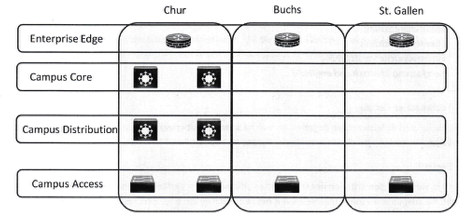
\includegraphics{Netzwerkstruktur.png}
\caption{Netzwerkstruktur}
\label{abb: Netzwerksturktur}
\end{figure}
\newpage

\section{Konzept}
\subsection{Ipv4 Adresskonzept} 
Das folgende Konzept gilt nur für IPv4, immer wenn von Adressen die Rede ist, sind nur IPv4 Adressen gemeint.
Für das private Netz werde Adressen aus dem 10.0.0.0/8 Netz ausgewählt. Für jeden Standort und für die Netze welche nicht einem Standort zugeornet werden können wird ein /16 Netz ausgewählt, so hat jeder Standort 65534 Ip-Adressen. Dies sollte für die nahe Zukunft genügen.\\
\newline
Die Aufteilung sieht folgendermassen aus: \\
\newline
\hspace*{1cm} 
\begin{tabular}{ll}
    Chur & 10.\colorbox{green}{1}.0.0/16\\
    St. Gallen & 10.\colorbox{green}{2}.0.0/16\\
    Buchs & 10.\colorbox{green}{3}.0.0/16\\
    Transfer & 10.\colorbox{green}{4}.0.0/16\\
\end{tabular}\\
\newline
Für die Vlans werden die Netze der Standorte nochmals unterteilt, die gelben Sterne im Vlan-Plan stehen für die Standorte. Mit /24 Netzen stehen jeder Abteilund pro Standort 256 Adressen zur Verfügung.\\
\newline
\hspace*{1cm} 
\begin{tabular}{lll}
     Vlan 10 & Geschäftsleitung & 10.\colorbox{yellow}{*}.\colorbox{green}{10}.0/24\\
     Vlan 20 & Buchhaltung & 10.\colorbox{yellow}{*}.\colorbox{green}{20}.0/24\\
     Vlan 30 & Entwicklung & 10.\colorbox{yellow}{*}.\colorbox{green}{30}.0/24\\
             & Transfer & 10.\colorbox{yellow}{*}.\colorbox{green}{40}.0/24\\
     Vlan 99 & Management & 10.\colorbox{yellow}{*}.\colorbox{green}{99}.0/24\\
\end{tabular}
\newpage
\subsection{Ipv6 Adresskonzept} 
Das folgende Konzept gilt nur für IPv6, immer wenn von Adressen die Rede ist, sind nur IPv6 Adressen gemeint.
Die Aufgabenstellung besagt, dass ein /48 Netz zur Verfügung steht, das Ziel ist nun dies in einer ähnlichen Art wie bei IPv4 zu gestalten. \\
\newline
Standortabhängigkeiten:\\ 
\newline
\hspace*{1cm} 
\begin{tabular}{ll}
    Chur & 2001:620:3101:\colorbox{green}{1}::/64\\
    St. Gallen & 2001:620:3101:\colorbox{green}{2}::/64\\
    Buchs & 2001:620:3101:\colorbox{green}{3}::/64\\
\end{tabular}\\
\newline
Da es bei IPv6 keine Vlans gibt, sondern alles über Layer-3, sprich IP, geschieht. Muss auch ein “Vlan-Konzept” für IPv6 erstellt werden. Dies wird analog zu IPv4 gemacht. Die gelben Sterne stehen für die Standortadresse.\\\newline
Netze der Abteilungen: \\
\newline
\hspace*{1cm} 
\begin{tabular}{lll}
     Vlan 10 & Geschäftsleitung & 2001:620:3101:\colorbox{yellow}{*}\colorbox{green}{010}::/64\\
     Vlan 20 & Buchhaltung & 2001:620:3101:\colorbox{yellow}{*}\colorbox{green}{020}::/64\\
     Vlan 30 & Entwicklung & 2001:620:3101:\colorbox{yellow}{*}\colorbox{green}{030}::/64\\
             & Transfer & 2001:620:3101:\colorbox{yellow}{*}\colorbox{green}{040}::/64\\
     Vlan 99 & Management & 2001:620:3101:\colorbox{yellow}{*}\colorbox{green}{099}::/64\\
\end{tabular}
\newpage



\subsection{Routingkonzept} 
Innerhalb unseres Unternehmens werden die verschiedenen Standorte miteinander über OSPF geroutet. Am Hauptstandort in Chur wird ab dem Distributions-Switch (D) ebenfalls mit OSPF geroutet. Beim Interface mit dem Internetanschluss wird eine default-Route gesetzt, da diese immer die Gleiche ist. Damit die Clients immer den gleichen default-Gateway haben, ist auf R1 noch ein Loopback-Interface erstellt worden, dieses darf nicht vergessen werden bei der Konfiguration von OSPF.
\subsection{NAT Konzept}
Meistens ist es für ein Unternehmen nicht rentabel sich die gesamte Anzahl benötigter IP-Adressen zu  kaufen. Deshalb werden private IP-Adressen verwendet und danach können mit einem NAT ganze Subnetze zu einer öffentlichen Adresse zugeordnet werden. Dies ist eine komfortable Lösung, ausserdem können dann die privaten Adressen so gestaltet werden, dass man nur schon beim anschauen weiss an welchem Standort und zu welchem Vlan die Adresse gehört.

\subsubsection{IPv4}
Für die öffentlichen Adressen steht ein /28 Netz zur Verfügung. Für die Verwendung von NAT können alle Adressen des Netzes benutzt werden, die Netz- und Broadcast-Adresse werden nicht benötigt. Somit stehen 16 öffentliche Adressen zur Benutzung, hier wurde für jeden Vlan an jedem Standort eine eigene Adresse verteilt. Dies ergibt 12 Adressen, die restlichen 4 Adressen sind für Reserven eingeplant.

\subsubsection{IPv6}
Bei IPv6 ist kein NAT notwendig, da ein öffentliches /48 Netz gebraucht wird. Es sind also mehr Adressen vorhanden als je in diesem Kleinunternehmen gebraucht werden.

\newpage
\subsection{Securitykonzept} 
\subsubsection{ACL}
Mit ACL's wird der Zugriff der Abteilungen untereinander verhindert, lediglich das Management-Vlan hat auf alles Zugriff, da dies für die reibungslose Verwaltung des Netzes erforderlich ist.
Die ACL's werden auf den Routern R2, R3 und auf dem Switch D konfiguriert, für die 3 Vlans der Abteilungen wird je der Zugriff der anderen Vlans verboten, danach werden alle anderen IP und TCP Pakete erlaubt. Dies wird für IPv4 und IPv6 gleich gemacht, als erstes wird eine ACL pro Vlan erstellt, danach wird diese ACL dem Vlan-Interface zugewiesen.

\subsubsection{Layer 2 Security}
\subsection{Serverservices}
\subsection{Netzwerkplan}
\section{Planung}
\section{Umsetzung}
\end{document}







